\section{Research Methodology}
\label{sec:Res}
\par This section is one of the most important parts of your research and it is the one that will receive most criticism. The reason is that here you document how you conducted your research. Since you are reading a B.Sc. degree you are expected to follow a scientific method, thus in this section you are expected to document: \textbf{the problem}; \textbf{hypothesis}; \textbf{aim \& objectives}; \textbf{research questions}; and \textbf{research pipeline}. Let's go through each.

\par Traditional interview are prone to bias and expenses to run an interview. With use of BART-MNLI, it prevents lacking qualitative depth of conversation while employing automated scoring based on required labels from open-ended answers. The research hyptohesized that \textit{there is a significant positive correlation between the semantic scores generated by the BART-MNLI model and the evaluation scores provided by expert human recruiters for the same set of open-ended responses.}

\par The primary aim of this reserach was to develop and make use of a simple python app that utilized Zero-Shot Natrual Language Processing to display real-time assesment of candidate personality traits based on open-ended responses.  Our research objectives were:
\begin{enumerate}
    \item Collect and simulate data set of open ended job interview responses related to specified employer skills 
    \item Implement BART-MNLI to generate a score for each user response
    \item Conduct correlation analysis between AI scores and human scores
    \item Measure and compare time taken to process automated scoring against time taken by human recruiters to evaluate users answers
    \item Conduct error analysis on instances with low correlation to detect linguistic issues or terms where ZSC fail to score.
\end{enumerate}

\par The research aimed to answer the following research questions:
\begin{enumerate}
    \item To what extent does the BART-MNLI zero-shot classification model correlate with expert human recruiter evaluations when scoring specific employer-required skills in open-ended interview responses?
    \item Does the use of automated NLI-based scoring significantly reduce the time required for the initial candidate screening phase compared to traditional human-led qualitative analysis?
    \item What are the primary linguistic limitations of the BART-MNLI model when interpreting nuanced or industry-specific terminology in candidate "stories"?
\end{enumerate}

\par Finally, you need a plan on how you intend to answer the research questions which will help you prove/disprove the hypothesis. Different research areas would require specific pipelines, yet a generic one is shown in Fig~\ref{fig:Pipeline}. After presenting an illustration of your pipeline it is recommended to documenting what has been done at every stage. Remember you should use past tense in this section since you are document what you have already done, since this paper will be published at the end of your research.

\begin{figure}[ht]
    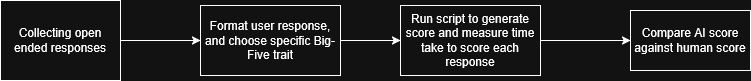
\includegraphics[scale=0.25]{includes/pipeline.png}
    \centering
    \caption{Research Pipeline}
    \label{fig:Pipeline}
\end{figure}